\documentclass[11pt]{article}
\usepackage{geometry}                
\geometry{letterpaper}
\usepackage[]{graphicx}
\usepackage{amssymb}
\usepackage{enumitem}
\usepackage{hyperref}
\usepackage{amsmath}
\usepackage{multicol}

%    Q-circuit version 2
%    Copyright (C) 2004  Steve Flammia & Bryan Eastin
%    Last modified on: 9/16/2011
%
%    This program is free software; you can redistribute it and/or modify
%    it under the terms of the GNU General Public License as published by
%    the Free Software Foundation; either version 2 of the License, or
%    (at your option) any later version.
%
%    This program is distributed in the hope that it will be useful,
%    but WITHOUT ANY WARRANTY; without even the implied warranty of
%    MERCHANTABILITY or FITNESS FOR A PARTICULAR PURPOSE.  See the
%    GNU General Public License for more details.
%
%    You should have received a copy of the GNU General Public License
%    along with this program; if not, write to the Free Software
%    Foundation, Inc., 59 Temple Place, Suite 330, Boston, MA  02111-1307  USA

% Thanks to the Xy-pic guys, Kristoffer H Rose, Ross Moore, and Daniel Müllner,
% for their help in making Qcircuit work with Xy-pic version 3.8.  
% Thanks also to Dave Clader, Andrew Childs, Rafael Possignolo, Tyson Williams,
% Sergio Boixo, Cris Moore, Jonas Anderson, and Stephan Mertens for helping us test 
% and/or develop the new version.

\usepackage{xy}
\xyoption{matrix}
\xyoption{frame}
\xyoption{arrow}
\xyoption{arc}

\usepackage{ifpdf}
\ifpdf
\else
\PackageWarningNoLine{Qcircuit}{Qcircuit is loading in Postscript mode.  The Xy-pic options ps and dvips will be loaded.  If you wish to use other Postscript drivers for Xy-pic, you must modify the code in Qcircuit.tex}
%    The following options load the drivers most commonly required to
%    get proper Postscript output from Xy-pic.  Should these fail to work,
%    try replacing the following two lines with some of the other options
%    given in the Xy-pic reference manual.
\xyoption{ps}
\xyoption{dvips}
\fi

% The following resets Xy-pic matrix alignment to the pre-3.8 default, as
% required by Qcircuit.
\entrymodifiers={!C\entrybox}

\newcommand{\bra}[1]{{\left\langle{#1}\right\vert}}
\newcommand{\ket}[1]{{\left\vert{#1}\right\rangle}}
    % Defines Dirac notation. %7/5/07 added extra braces so that the commands will work in subscripts.
\newcommand{\qw}[1][-1]{\ar @{-} [0,#1]}
    % Defines a wire that connects horizontally.  By default it connects to the object on the left of the current object.
    % WARNING: Wire commands must appear after the gate in any given entry.
\newcommand{\qwx}[1][-1]{\ar @{-} [#1,0]}
    % Defines a wire that connects vertically.  By default it connects to the object above the current object.
    % WARNING: Wire commands must appear after the gate in any given entry.
\newcommand{\cw}[1][-1]{\ar @{=} [0,#1]}
    % Defines a classical wire that connects horizontally.  By default it connects to the object on the left of the current object.
    % WARNING: Wire commands must appear after the gate in any given entry.
\newcommand{\cwx}[1][-1]{\ar @{=} [#1,0]}
    % Defines a classical wire that connects vertically.  By default it connects to the object above the current object.
    % WARNING: Wire commands must appear after the gate in any given entry.
\newcommand{\gate}[1]{*+<.6em>{#1} \POS ="i","i"+UR;"i"+UL **\dir{-};"i"+DL **\dir{-};"i"+DR **\dir{-};"i"+UR **\dir{-},"i" \qw}
    % Boxes the argument, making a gate.
\newcommand{\meter}{*=<1.8em,1.4em>{\xy ="j","j"-<.778em,.322em>;{"j"+<.778em,-.322em> \ellipse ur,_{}},"j"-<0em,.4em>;p+<.5em,.9em> **\dir{-},"j"+<2.2em,2.2em>*{},"j"-<2.2em,2.2em>*{} \endxy} \POS ="i","i"+UR;"i"+UL **\dir{-};"i"+DL **\dir{-};"i"+DR **\dir{-};"i"+UR **\dir{-},"i" \qw}
    % Inserts a measurement meter.
    % In case you're wondering, the constants .778em and .322em specify
    % one quarter of a circle with radius 1.1em.
    % The points added at + and - <2.2em,2.2em> are there to strech the
    % canvas, ensuring that the size is unaffected by erratic spacing issues
    % with the arc.
\newcommand{\measure}[1]{*+[F-:<.9em>]{#1} \qw}
    % Inserts a measurement bubble with user defined text.
\newcommand{\measuretab}[1]{*{\xy*+<.6em>{#1}="e";"e"+UL;"e"+UR **\dir{-};"e"+DR **\dir{-};"e"+DL **\dir{-};"e"+LC-<.5em,0em> **\dir{-};"e"+UL **\dir{-} \endxy} \qw}
    % Inserts a measurement tab with user defined text.
\newcommand{\measureD}[1]{*{\xy*+=<0em,.1em>{#1}="e";"e"+UR+<0em,.25em>;"e"+UL+<-.5em,.25em> **\dir{-};"e"+DL+<-.5em,-.25em> **\dir{-};"e"+DR+<0em,-.25em> **\dir{-};{"e"+UR+<0em,.25em>\ellipse^{}};"e"+C:,+(0,1)*{} \endxy} \qw}
    % Inserts a D-shaped measurement gate with user defined text.
\newcommand{\multimeasure}[2]{*+<1em,.9em>{\hphantom{#2}} \qw \POS[0,0].[#1,0];p !C *{#2},p \drop\frm<.9em>{-}}
    % Draws a multiple qubit measurement bubble starting at the current position and spanning #1 additional gates below.
    % #2 gives the label for the gate.
    % You must use an argument of the same width as #2 in \ghost for the wires to connect properly on the lower lines.
\newcommand{\multimeasureD}[2]{*+<1em,.9em>{\hphantom{#2}} \POS [0,0]="i",[0,0].[#1,0]="e",!C *{#2},"e"+UR-<.8em,0em>;"e"+UL **\dir{-};"e"+DL **\dir{-};"e"+DR+<-.8em,0em> **\dir{-};{"e"+DR+<0em,.8em>\ellipse^{}};"e"+UR+<0em,-.8em> **\dir{-};{"e"+UR-<.8em,0em>\ellipse^{}},"i" \qw}
    % Draws a multiple qubit D-shaped measurement gate starting at the current position and spanning #1 additional gates below.
    % #2 gives the label for the gate.
    % You must use an argument of the same width as #2 in \ghost for the wires to connect properly on the lower lines.
\newcommand{\control}{*!<0em,.025em>-=-<.2em>{\bullet}}
    % Inserts an unconnected control.
\newcommand{\controlo}{*+<.01em>{\xy -<.095em>*\xycircle<.19em>{} \endxy}}
    % Inserts a unconnected control-on-0.
\newcommand{\ctrl}[1]{\control \qwx[#1] \qw}
    % Inserts a control and connects it to the object #1 wires below.
\newcommand{\ctrlo}[1]{\controlo \qwx[#1] \qw}
    % Inserts a control-on-0 and connects it to the object #1 wires below.
\newcommand{\targ}{*+<.02em,.02em>{\xy ="i","i"-<.39em,0em>;"i"+<.39em,0em> **\dir{-}, "i"-<0em,.39em>;"i"+<0em,.39em> **\dir{-},"i"*\xycircle<.4em>{} \endxy} \qw}
    % Inserts a CNOT target.
\newcommand{\qswap}{*=<0em>{\times} \qw}
    % Inserts half a swap gate.
    % Must be connected to the other swap with \qwx.
\newcommand{\multigate}[2]{*+<1em,.9em>{\hphantom{#2}} \POS [0,0]="i",[0,0].[#1,0]="e",!C *{#2},"e"+UR;"e"+UL **\dir{-};"e"+DL **\dir{-};"e"+DR **\dir{-};"e"+UR **\dir{-},"i" \qw}
    % Draws a multiple qubit gate starting at the current position and spanning #1 additional gates below.
    % #2 gives the label for the gate.
    % You must use an argument of the same width as #2 in \ghost for the wires to connect properly on the lower lines.
\newcommand{\ghost}[1]{*+<1em,.9em>{\hphantom{#1}} \qw}
    % Leaves space for \multigate on wires other than the one on which \multigate appears.  Without this command wires will cross your gate.
    % #1 should match the second argument in the corresponding \multigate.
\newcommand{\push}[1]{*{#1}}
    % Inserts #1, overriding the default that causes entries to have zero size.  This command takes the place of a gate.
    % Like a gate, it must precede any wire commands.
    % \push is useful for forcing columns apart.
    % NOTE: It might be useful to know that a gate is about 1.3 times the height of its contents.  I.e. \gate{M} is 1.3em tall.
    % WARNING: \push must appear before any wire commands and may not appear in an entry with a gate or label.
\newcommand{\gategroup}[6]{\POS"#1,#2"."#3,#2"."#1,#4"."#3,#4"!C*+<#5>\frm{#6}}
    % Constructs a box or bracket enclosing the square block spanning rows #1-#3 and columns=#2-#4.
    % The block is given a margin #5/2, so #5 should be a valid length.
    % #6 can take the following arguments -- or . or _\} or ^\} or \{ or \} or _) or ^) or ( or ) where the first two options yield dashed and
    % dotted boxes respectively, and the last eight options yield bottom, top, left, and right braces of the curly or normal variety.  See the Xy-pic reference manual for more options.
    % \gategroup can appear at the end of any gate entry, but it's good form to pick either the last entry or one of the corner gates.
    % BUG: \gategroup uses the four corner gates to determine the size of the bounding box.  Other gates may stick out of that box.  See \prop.

\newcommand{\rstick}[1]{*!L!<-.5em,0em>=<0em>{#1}}
    % Centers the left side of #1 in the cell.  Intended for lining up wire labels.  Note that non-gates have default size zero.
\newcommand{\lstick}[1]{*!R!<.5em,0em>=<0em>{#1}}
    % Centers the right side of #1 in the cell.  Intended for lining up wire labels.  Note that non-gates have default size zero.
\newcommand{\ustick}[1]{*!D!<0em,-.5em>=<0em>{#1}}
    % Centers the bottom of #1 in the cell.  Intended for lining up wire labels.  Note that non-gates have default size zero.
\newcommand{\dstick}[1]{*!U!<0em,.5em>=<0em>{#1}}
    % Centers the top of #1 in the cell.  Intended for lining up wire labels.  Note that non-gates have default size zero.
\newcommand{\Qcircuit}{\xymatrix @*=<0em>}
    % Defines \Qcircuit as an \xymatrix with entries of default size 0em.
\newcommand{\link}[2]{\ar @{-} [#1,#2]}
    % Draws a wire or connecting line to the element #1 rows down and #2 columns forward.
\newcommand{\pureghost}[1]{*+<1em,.9em>{\hphantom{#1}}}
    % Same as \ghost except it omits the wire leading to the left. 


\begin{document}

\begin{center}
    {\LARGE Project Proposal: A classical simulator\\ for quantum circuits dominated by Clifford gates }
\vspace{2mm}
{\large \\ Patrick Rall and Iskren Vankov, advised by David Gosset \\ California Institute of Technology -  \today}
\end{center}

%figure environment for multicols
\newenvironment{Figure}
  {\par\medskip\noindent\minipage{\linewidth}}
  {\endminipage\par\medskip}


\begin{multicols}{2}

\subsection*{Introduction}
Simulation of quantum circuits on classical computers is a useful tool for the verification and validation of quantum devices. As we build systems with more and more qubits, we will enter a regime where simulation will become impractical. While this is a central reason for our interest in quantum devices, extending the reach of classical computers for verification purposes will have practical applications in experiments conducted in the near future.

A recent paper by Sergey Bravyi and David Gosset \cite{bravyi-gosset} describes an algorithm for quantum circuit simulation that is polynomial in the number of qubits. By utilizing the Gottesmann-Knill theorem to efficiently simulate Clifford gates, the procedure is only exponential in the number of $T$-gates used in the circuit. A preliminary Matlab implementation was capable of simulating a hidden shift quantum algorithm with 40 qubits and 50 $T$-gates on a laptop.

The goal of this project is to develop an open-source application that permits other physicists to use this algorithm. It will employ a massively parallel architecture, so it can be run on hundreds of CPUs in a computer cluster. It will also be able to make use of Graphics Processing Units (GPUs) present in many laptops and desktops, which could be useful for physicists with limited access to a cluster. 

In addition to creating a useful tool, this project will be an excellent learning experience. We will learn more about the inner workings of the Gottesmann-Knill theorem, stabilizer states, and mathematical tools used in modern quantum information science. We will also gain experience in writing distributed software for several architectures, and how to automatically manage highly parallel code across many computers. 


\subsection*{Algorithm sketch}

\begin{Figure}
\[ \Qcircuit @C=1em @R=.7em {
& \gate{T} &  \qw }  =  
\Qcircuit @C=1.3em @R=.6em {
  & \qw & \qw & \ctrl{1} & \qw & \gate{S} & \qw \\
  & & \lstick{\ket{A}} & \targ \qw & \meter & \cw \cwx  
} \]
Figure 1: The $T$-gate gadget. By replacing all occurrences of $T$ with this gadget we can avoid using non-Clifford gates in the simulation. However, we now require several non-stabilizer states $\ket{A} =\frac{1}{\sqrt{2}} (\ket{0} + e^{i\pi/4}\ket{1})$. 
\end{Figure}

The paper \cite{bravyi-gosset} describes two algorithms. An algorithm for computing the output probability of a string $x$ runs in
    $$ \text{poly}(n,m) + 2^{0.5t} t^3. $$
    Another algorithm for sampling a string $x$ from the output distribution runs in
    $$ \text{poly}(n,m) + 2^{0.23t}t^3 w^4,$$
    where $n$ is the number of qubits, $m$ the total number of gates, $t$ the number of $T$-gates and $w$ the size of the string $x$.

\clearpage

\begin{itemize}
\setlength{\itemsep}{0em} %reduce spacing 
    \item Both algorithms replace all occurrences of the $T$-gate with the gadget shown in Figure 1, so a Clifford-only circuit must be simulated.
    \item Each $T$-gate gadget consumes a non-stabilizer `magic state':
    $$\ket{A} =\frac{1}{\sqrt{2}} (\ket{0} + e^{i\pi/4}\ket{1}).$$ Thus the circuit requires an additional $\ket{A}^{\otimes t}$ state.
    \item The state $\ket{A}^{\otimes t}$ is decomposed into a linear combination of $\chi \ll 2^n$ stabilizer states.
    \item The action of the circuit onto each stabilizer state in this linear combination can be computed independently. This is why parallelism is so appropriate for this algorithm.
    \item The final measurements are also performed independently on each resulting state in the linear combination.
    \item Computing the norm of the final state can be achieved in $O(\chi t^3 \epsilon^{-2})$ for relative error $\epsilon$. \textbf{Can this procedure be parallelized too?}
\end{itemize}


\subsection*{Software architecture}


\begin{description}
    \item[Scheduler, Network Manager] (Python) \\
        The heart of the application will perform all tasks that cannot be done in parallel. It will network together all computers that will perform computation and scan for computing resources. It will decompose the $\ket{A}^{\otimes t}$ state into $\chi$ stabilizer states and assign them to the available resources. Once parallel computation is complete it will normalize the resulting state and produce the final output.
    \item[CPU Simulator] (C++) \\
        A simple implementation of a stabilizer circuit simulator for a single state, aimed for high performance on a single CPU core.
    \item[GPU Simulator] (CUDA) \\
        A highly parallel implementation of a stabilizer circuit simulator for several states. This component must be capable of adapting to a range of GPUs with different capabilities.
    \item[Command Line Interface] (Python) \\
        A simple tool capable of reading circuits from a file, starting the simulation, and presenting the result.
    \item[Web Interface] (Python, Javascript) \\
        A web server providing a graphical user interface. It provides a tool for entering circuits \textbf{(maybe using LIQUID?)}, simulating them on demand, and gathering statistics for the results.
\end{description}

\begin{Figure}
\hspace{0.1in}
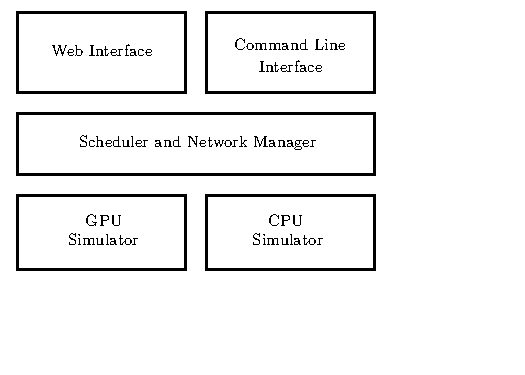
\includegraphics{diagrams/architecture.pdf}

\vspace{-0.5in}

{Figure 2: Software architecture for the simulator. The project is split into five modules described above.}
\end{Figure}

\clearpage

\end{multicols}

\subsection*{Time plan}
\begin{description}
    \item[Before Spring Term] We will read papers, regularly meet with David Gosset, and solidify our understanding of the algorithms. We will study GPU programming and evaluate challenges and limitations in building a parallel stabilizer circuit simulator.
    \item[March] An initial implementation of a stabilizer circuit simulator in C++ should be written during spring break. That way if there are any questions on how to proceed we can immediately dive into details when term begins and regular meetings resume. Spring term begins March 28. The last week of March should be dedicated to implementing the algorithms in \cite{bravyi-gosset} in python, utilizing the working stabilizer circuit simulator.
    \item[April] April will be dedicated to building the GPU simulator, which will be unfamiliar territory for both participants. Iskren will be taking \textit{CS179 GPU Programming} (textbook: \cite{cudahandbook}) and will be able to contribute with knowledge from the class. Both of us are experienced with the `dive in at the deep end and figure out how to swim'-approach to coding.
    \item[May] On May 2 David Gosset \textbf{will leave Caltech (how accurate is this?)}, so the physics of the algorithm must be working in all parts of the code by then. May will be spent writing the command line interface and web interface, as well as documenting and polishing the code. We will request time on Caltech's compute cluster to test the algorithm. 
    \item[June] The last weeks of term will be spent completing and polishing the documentation. Commencement is June 10.

\end{description}





\begin{thebibliography}{2}
    \bibitem{bravyi-gosset} S. Bravyi, D. Gosset. Jan 29, 2016. ``Improved classical simulation of quantum circuits dominated by Clifford gates''. \url{http://arxiv.org/abs/1601.07601}
    \bibitem{bravyi-smith-smolin} S. Bravyi, G. Smith, J. Smolin. Jun 3, 2015. ``Trading classical and quantum computational resources''. \url{http://arxiv.org/abs/1506.01396}
    \bibitem{gottesman-aaronson} A. Aaronson, D. Gottesman. Jun 25 2004. ``Improved Simulation of Stabilizer Circuits''. \url{http://arxiv.org/abs/quant-ph/0406196}
    \bibitem{cudahandbook} N. Wilt. Jun 12, 2013, Addison-Wesley Professional. ``The CUDA Handbook: A Comprehensive Guide to GPU Programming''. \url{http://www.cudahandbook.com/}
\end{thebibliography}

\end{document}

